\documentclass[11pt,twoside]{article}
\usepackage{geometry}
\usepackage{enumerate}
\usepackage{latexsym,booktabs}
\usepackage{amsmath,amssymb}
\usepackage{graphicx}
\usepackage[colorlinks, linkcolor = blue]{hyperref}
\usepackage[singlespacing]{setspace}
\usepackage{calc}
\usepackage{multirow}


\geometry{a4paper,left=2cm,right=2.0cm, top=2cm, bottom=2.0cm}

\newtheorem{Definition}{Definition}
\newtheorem{Theorem}{Theorem}
\newtheorem{Lemma}{Lemma}
\newtheorem{Corollary}{Corollary}
\newtheorem{Proposition}{Proposition}
\newtheorem{Algorithm}{Algorithm}
\numberwithin{Theorem}{section}
\numberwithin{Definition}{section}
\numberwithin{Lemma}{section}
\numberwithin{Algorithm}{section}
\numberwithin{equation}{section}

\newcommand{\dottedline}[1]{\makebox[#1]{.\dotfill}}

\begin{document}
	
\pagestyle{empty}

 %=============================================================================
 %Title page
 %=============================================================================
\begin{titlepage}
\vspace*{.5em}
\centering
\textbf{\Large{The School of Mathematics}} \\
\vspace*{1em}
\begin{figure}[!h]
\centering

\includegraphics[width=180pt]{CentredLogoCMYK.jpg}
\end{figure}
\vspace{2em}
\textbf{\Huge{Analysis on Leptospirosis Risk Factors Based on General Linear Mixed Models}}\\[2em]
\textbf{\LARGE{by}}\\
\vspace{2em}
\textbf{\LARGE{Yile Shi}}\\
\vspace{6.5em}
\Large{Dissertation Presented for the Degree of\\
MSc in Statistics with Data Science}\\
\vspace{6.5em}
\Large{August 2021}\\
\vspace{3em}
\Large{Supervised by\\Dr. Gail Robertson and Dr. Amy Wilson}
\vfill
\end{titlepage}

\clearpage

% =============================================================================
% Executive summary, acknowledgments, and own work declaration
% =============================================================================
\begin{center}
\Large{Executive Summary}
\end{center}

\textbf{Background:} Leptospirosis, a widely distributed zoonotic disease in both developed and developing countries, has become a major public health concern due to its significant effect on human and animal morbidity and mortality \cite{haake2015leptospirosis}. Although various researches have been conducted to study this zoonotic infection in different domains, work on identifying individuals at risk, especially in low-income rural areas in developing countries, is still deficient.

\

\textbf{Research question:} This research aims to shed light on the potential risk factors that affects leptospirosis infection in a rural area of Kenya, and further generate knowledge to help inform health intervention programmes for leptospirosis infections reduction. We consider 8 demographic variables: gender, age, land use, occupation, distance to local hospital, altitude, family size, and occupation of household head, as well as 3 environmental variables including village, location and constituency.

\

\textbf{Data:} We use the dataset which consists of 595 samples collected by the International Livestock Research Institute from members of households in villages in Tana River County, Kenya, including the Leptospirosis test results using ELIZA (enzyme-linked immunosorbent assay) and aforementioned variables.


\

\textbf{Methods:} We construct binomial General Linear Mixed Models including the random effect of environmental variables, where the response of interest is individual's ELIZA test result. The random intercept model with village effect is selected due to its best performance by AIC (Akaike Information Criterion). Further, we conduct model diagnosis and evaluation including ROC (Receiver Operating Characteristic) curves (Figure \ref{fig:ROC}) and AUC (Area Under Curve).

\

\textbf{Results:} Gender, type of land use and occupation of household head are shown to have significant effects on individual's Leptospirosis infection. Specifically, males

\begin{figure}[!h]
	\centering
	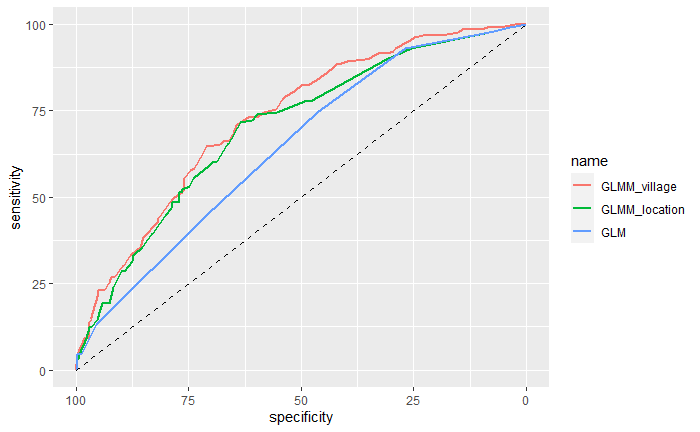
\includegraphics[width = 0.75\textwidth]{Images/ROC.png}
	\caption{ROC curves of different models}
	\label{fig:ROC}
\end{figure}

\clearpage

\begin{center}
\Large{Acknowledgments}
\end{center}

I am sincerely grateful to the supervisors of this project, Dr. Sara Wade and Dr. Cecilia Balocchi, as well as PhD supporter Steven Soutar, for their advice and guidance. I would also like to thank SHARE for providing the data and background information used in the research. 


\clearpage


\begin{center}
\Large{University of Edinburgh – Own Work Declaration}
\end{center}

This sheet must be filled in, signed and dated - your work will not be marked unless this is done.
\vspace{1cm}

Name: Yile Shi

Matriculation Number: s2168022

Title of work: Analysis on Dementia Risk Factors Based on Bayesian Networks

\vspace{1cm}

We confirm that all this work is my own except where indicated, and that We have:
\begin{itemize}
\item	Clearly referenced/listed all sources as appropriate	 				
\item	Referenced and put in inverted commas all quoted text (from books, web, etc)	
\item	Given the sources of all pictures, data etc. that are not my own				
\item	Not made any use of the report(s) or essay(s) of any other student(s) either past 	
or present	
\item	Not sought or used the help of any external professional academic agencies for the work
\item	Acknowledged in appropriate places any help that We have received from others	(e.g. fellow students, technicians, statisticians, external sources)
\item	Complied with any other plagiarism criteria specified in the Course handbook
\end{itemize}

We understand that any false claim for this work will be penalised in accordance with
the University regulations	(\url{https://teaching.maths.ed.ac.uk/main/msc-students/msc-programmes/statistics/data-science/assessment/academic-misconduct}).								

\vspace{1cm}

Signature:

\begin{figure}[!h]
	
\includegraphics[width = 0.5\textwidth]{Images/Signature.png}
\end{figure}

\vspace{5mm}

Date: 2022/8/10

\clearpage


% =============================================================================
% Table of contents, tables, and pictures (if applicable)
% =============================================================================
\pagestyle{plain}
\setcounter{page}{1}
\pagenumbering{Roman}

\tableofcontents

\pagenumbering{arabic}
\setcounter{page}{1}

\nocite{*}
\bibliographystyle{unsrt}
\clearpage

\section{Introduction}
\label{sec:intro}

Dementia, a clinical state characterized by loss of function in multiple cognitive domains, becomes a serious public health concern worldwide \cite{seixas2014bayesian}. Someone develops dementia every 3 seconds and current annual cost of dementia is estimated at 1 million dollars, which is set double in 2030 \cite{alzheimer2019world}. Because of the absence of effective treatment, prevention strategy to reduce dementia risk becomes an active research topic. This report aims to contribute to this topic by identifying potential risk factors behind dementia diagnosis. We expect that a better understanding of the influence of factors on cognitive impairment can help to inform the development of lifestyle interventions for dementia risk reduction. 

We apply exploratory data analysis on easySHARE dataset from Survey of Health, Ageing and Retirement in Europe (SHARE) and extract a sample of 57310 individuals recorded in 2013. Based on the subset, we build Bayesian networks and select the one with the best performance. Our goal is to find, among the following factors, the most likely to be relevant to cognitive decline: age; gender; country; education; drinking behaviour; smoking; obesity; physical activity; chronic disease; working status; household finance; social isolation; and depression. 

\clearpage

\section{Exploratory Data Analysis}  
\label{sec: EDA}

\subsection{Erroneous Data and Duplicated Data}

We start with going through the dataset to have some initial insight of the data and detect that there exist some fault data against our general knowledge. For example, according to the column \texttt{relationshiphh}, some sampled people are the daughters of their corresponding household heads while their genders are recoded as "Male". We fix these problems. Besides, we observe and drop some duplicated data which are possibly recorded by accident. 

Note that there also exist some pairs of observations that are different in \texttt{sampleid} and \texttt{parent} but have same values in other columns. We decide to keep both of them in the dataset as we cannot tell whether these observations are duplicated or not.  

\subsection{Missing Data}

Table \ref{tab:missing} displays the number and the proportion (4 decimal places) of missing values in variables, arranged in descending order. 

\begin{table}[!h]
	\centering
	\begin{tabular}{|c|c|c|}
		\hline
		variable & count & proportion \\
		\hline
		\texttt{occupation} & 343 & 0.3649 \\ 
		\texttt{disthosp} &259 & 0.2755 \\
		\texttt{livestk\_home}  &  236 & 0.2511 \\
        \texttt{location}  &  236 & 0.2511 \\
		\texttt{landuse} & 4 & 0.0043 \\
		\texttt{gender} & 1 & 0.0011 \\
		\texttt{age} & 1 & 0.0011 \\
		\hline
	\end{tabular}
	\caption{Number and proportion of missing values in variables}
	\label{tab:missing}
\end{table}

According to the table above, we find that \texttt{landuse}, \texttt{gender} and \texttt{age} contain missing values less than 1\%. Thus, we drop the corresponding observations as it doesn't lead to much loss of information of the original dataset.

As for \texttt{occupation}, \texttt{disthosp}, \texttt{livestk\_home} and \texttt{location}, which contains a large amount of missing data respectively, they require exploration and discussion in more detail to determine a proper way to deal with missing data.

\subsubsection{livestk\_home}

According to the data description, \texttt{livestk\_home} is a binary variable indicating whether or not livestock is kept in the household of sampled person. The work of Cook et al in 2017 \cite{cook2017risk} found that the exposure to livestocks could be an important risk factor for Leptospirosis, hence we might also expect the significant contribution to Leptospirosis diagnosis of this variable. However, from figure \ref{fig:livestk}, we observe a significant imbalance in this column where most families of sampled people have livestocks at their homes. In this case, we will not include this variable in further analysis as the imbalance probably leads to insignificant results of this variable. It becomes unnecessary to think of the missing values in this column.

\begin{figure}[!h]
	\centering
	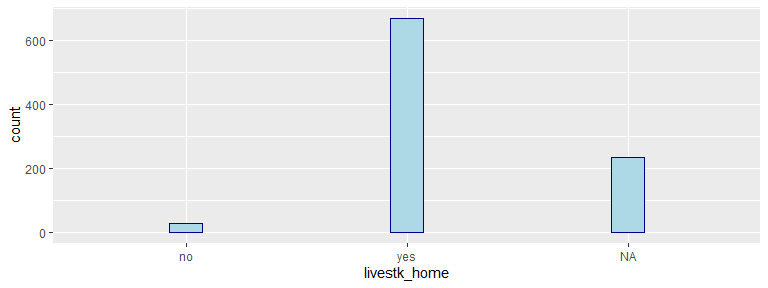
\includegraphics[width = 0.75\textwidth]{Images/livestk.png}
	\caption{Distribution of \texttt{livestk\_home}}
	\label{fig:livestk}
\end{figure}

\subsubsection{disthosp}

\texttt{disthosp} is the Euclidean distance from the sampled person's household to local hospital. Here, we assume that there is only one hospital in each village and people from that village only go to that hospital. Then, we use the mean distance to the local hospital of each village to impute the missing values in this column, which works for most villages. We observe that data in \texttt{disthosp} in village 12, 13 and 23 are completely missing, so we cannot obtain the mean distance to the local hospital and further fail to impute the missing distance in these villages. As a result, we drop the corresponding rows of village 12, 13 and 23.

\subsubsection{location}

\texttt{location} is the anonymised location of area where sampling was done, ranging from 1 to 19. This column has over 25\% missing data. Again, we consider using the \texttt{village} variable to determine the corresponding location in the same row. However, two problems are detected:

\begin{itemize}
	\item Similar to the case of \texttt{disthosp}, the locations of observations in some villages are completely missing, which makes it difficult to determine the correct locations.
	\item Some observations in the same village belong to different locations, e.g. some individuals from village 17 belong to location 9 while others belong to location 18. Without more information, we cannot decide which location they belong to, as it could be a mistake in data input or the corresponding village is on the boundary of two locations.
\end{itemize}

As a result, we drop all missing values in this column instead of imputation due to problems above.

\subsubsection{occupation}

The column \texttt{occupation} represents the occupation of the person sampled, which could have influence on the prevalence of Leptospirosis. Specifically, \cite{cook2017risk} pointed out that people whose working places are closer to water or animals are more likely to suffer from Leptospirosis. Therefore, we may want to take this variable into consideration when modelling and deal with this column more carefully. 

The occupation of a person could be associated with various aspects. We first consider the influence of individual's age. Figure \ref{fig:occ1} and \ref{fig:occ2} show the conditional distributions of \texttt{occupation} in juvenile (< 18 yeas old) and adult ($\geq$ 18 years old) groups respectively. 

\begin{figure}[!h]
	\centering
	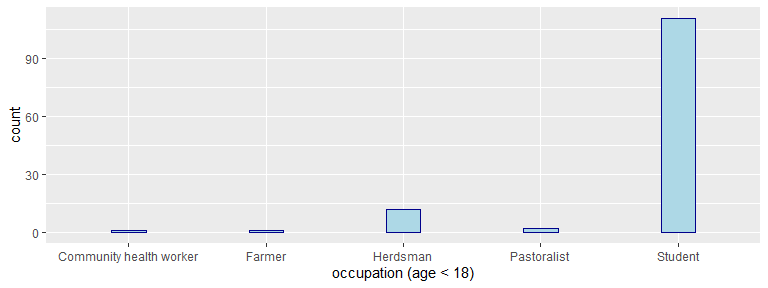
\includegraphics[width = 0.75\textwidth]{Images/occupation_age_1.png}
	\caption{Distribution of \texttt{occupation} in juvenile group}
	\label{fig:occ1}
\end{figure}

\begin{figure}[!h]
	\centering
	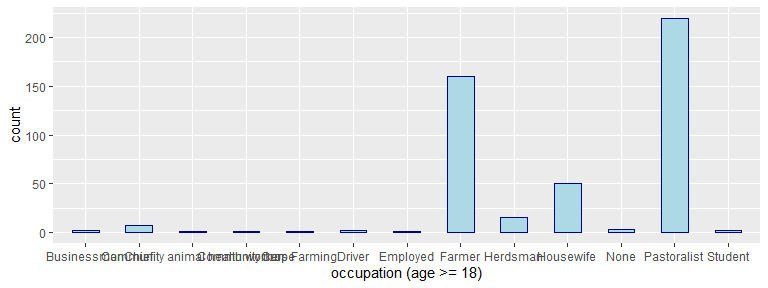
\includegraphics[width = 0.75\textwidth]{Images/occupation_age_2.png}
	\caption{Distribution of \texttt{occupation} in adult group}
	\label{fig:occ2}
\end{figure}

We observe very different distributions in two groups from the plots. For juveniles under 18 years old, they are most likely to be students, hence we impute the missing occupation for juvenile individuals with "Student", which is consistent with our general knowledge.  

The case for adults is more complex, as their occupations are also correlated with other variables. \texttt{landuse} denotes the characterization of the sampling site based on land use, which might be correlated with individual's occupation. Figure \ref{fig:occ3} displays the conditional distributions of adults' occupations in different \texttt{landuse} groups.

\begin{figure}[!h]
	\centering
	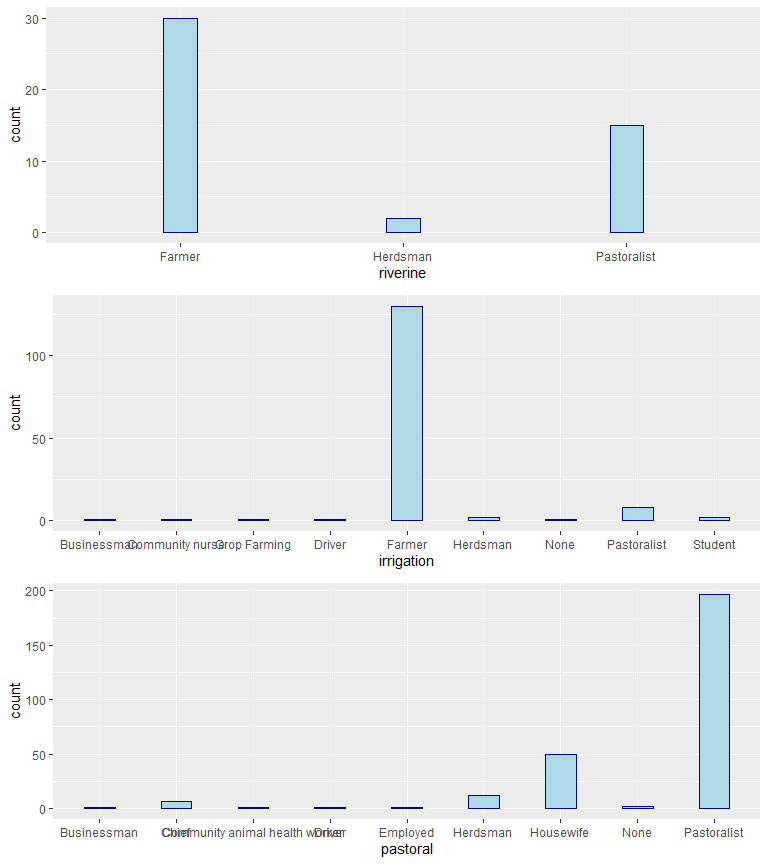
\includegraphics[width = 0.75\textwidth]{Images/occupation_landuse.png}
	\caption{Conditional distributions of \texttt{occupation} in adult group}
	\label{fig:occ3}		
\end{figure} 

According to the plot, most sampled adults with land use as "riverine" or "irrigation" work as farmers, while individuals with land use as "pastoral" are most likely to be pastoralists. Moreover, holding the \texttt{landuse} as "pastoral", we observe significance difference among different gender and constituency groups, as shown in Figure \ref{fig:occ4}.

\begin{figure}[!h]
	\centering
	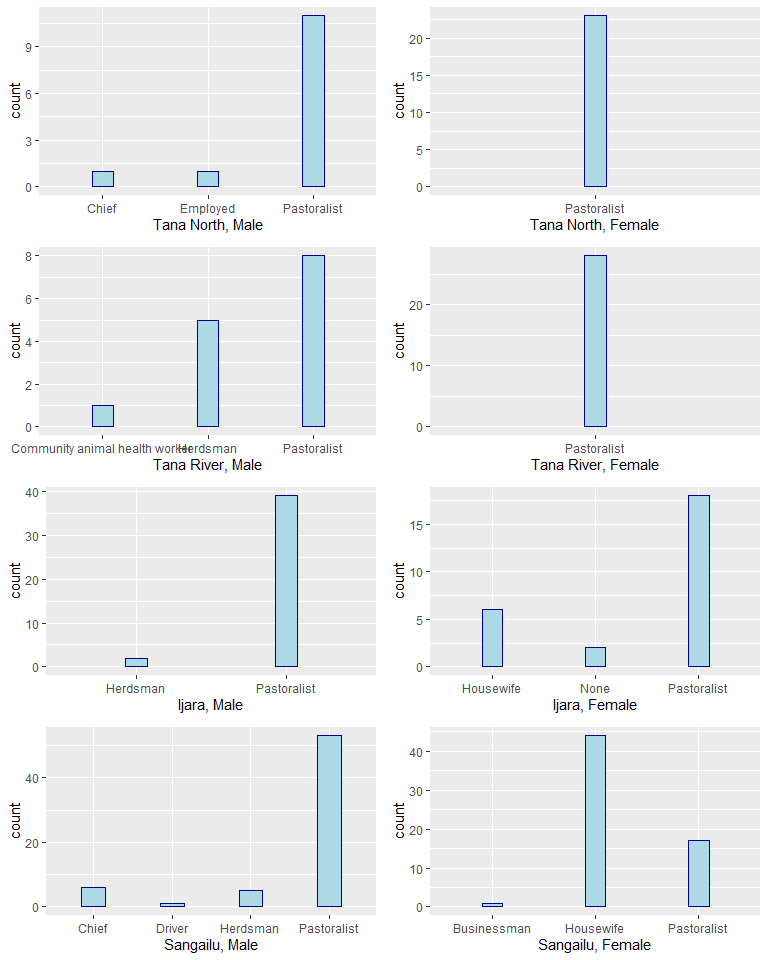
\includegraphics[width = 0.75\textwidth]{Images/occupation_gender_constituency.png}
	\caption{Conditional distributions of \texttt{occupation} in adult and "pastoral" group}
	\label{fig:occ4}		
\end{figure} 

In the "pastoral" stratification, male individuals across constituencies usually have their occupations as "Pastoralist", while female groups show various distributions. Females from "Tana North" and "Tana River" constituencies all work as pastoralists, but some of those from "Ijara" and "Sangailu" constituencies are housewives. Note that "Housewife" is the most popular occupation in "Sangailu" constituency, rather than "Pastoralist".

Therefore, we decide to drop observations with missing values in \texttt{occupation} instead of imputing them, as the cases are complicated and imputations probably lead to great model bias. 

\subsection{Feature Selection}

After dealing with missing data, we now determine which columns could be used for modelling. The column \texttt{result}, which represents whether the sample is positive or negative on ELISA (enzyme-linked immunosorbent assay), is considered as the response variable in our model. 

As for potential risk factors, according to the data description, identifier columns including \texttt{sampleid} and \texttt{parent} are excluded from our model, as well as \texttt{relationshiphh} and \texttt{genhhid}. Besides, as mentioned before, we do not take the variable \texttt{livestk\_home} into consideration. We select features from other columns based on corresponding plots and the work of Goarant et al (2016) \cite{goarant2016leptospirosis}. 

\subsubsection{Nominal Variables}

We start from factor variables \texttt{gender}, \texttt{occupation}, \texttt{landuse}, \texttt{hhoccup} and \texttt{hhgender}. The last two columns are nominal variables indicating the occupation and gender of the corresponding household head. Before any selection, we count the number of observations in each category of \texttt{occupation} and \texttt{hhoccup}. Moreover, we plot the stacked bars of \texttt{result}, grouped by these two columns respectively.

\begin{table}[!h]
	\centering
	\begin{tabular}{|l|l|l|l|}
		\hline
		\multicolumn{2}{|c|}{\texttt{occupation}} & \multicolumn{2}{|c|}{\texttt{hhoccup}} \\
		\hline
		category & 	count & category & count \\
		\hline
		Student & 239 & Pastoralist & 345 \\				
		Pastoralist & 159 & Farmer & 247 \\
		Farmer & 156 & Chief & 15 \\
		Housewife & 36	& Businessman & 5 \\			
		Herdsman & 20 & Civil Servant & 4 \\	
		Chief & 6 & Herdsman & 3 \\	
		Businessman & 2 & Crop Farming & 2 \\
		Driver & 2 & None & 2 \\
		Community animal health worker & 1 & Casual Labourer & 1 \\			
		Community nurse & 1	& Driver & 1 \\	
		Crop Farming & 1 & & \\			
		Employed & 1 & & \\
		None & 1 & & \\
		\hline
	\end{tabular}	
	\caption{Number of observations in each category in \texttt{occupation} and \texttt{hhoccup}}
	\label{tab:occ}
\end{table}

\begin{figure}[!h]
	\centering
	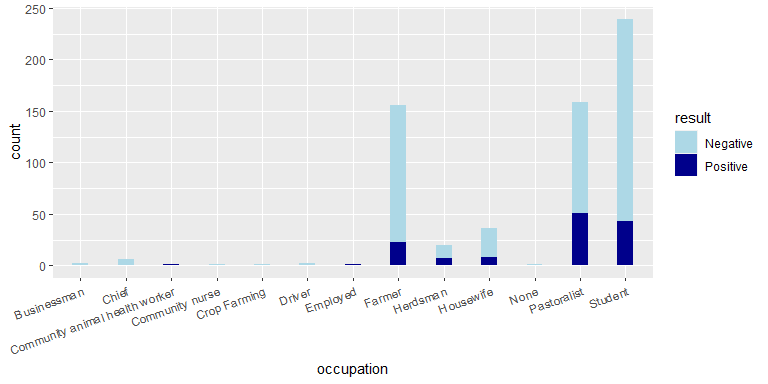
\includegraphics[width = 0.75\textwidth]{Images/occupation_3.png}
	\caption{Stacked bar plot of \texttt{result} in \texttt{occupation}}
	\label{fig:occ5}
\end{figure}

\begin{figure}[!h]
	\centering
	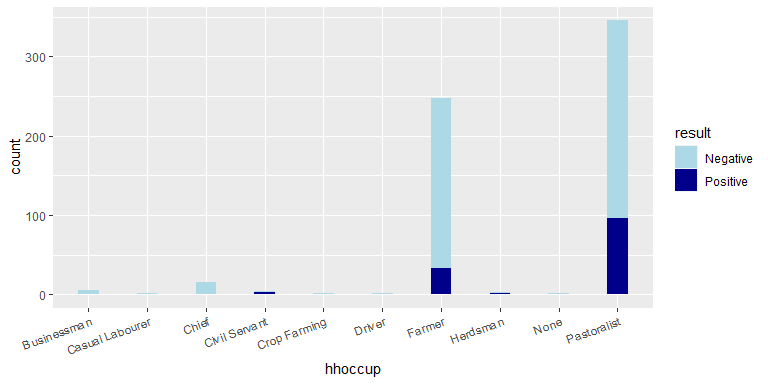
\includegraphics[width = 0.75\textwidth]{Images/hhoccup.png}
	\caption{Stacked bar plot of \texttt{result} in \texttt{hhoccup}}
	\label{fig:hhoccup}
\end{figure}

 According to Table \ref{tab:occ} and Figure \ref{fig:occ5} and \ref{fig:hhoccup}, most categories in two columns have observations less than 20. Small and insufficient group size would lead to unstable and  biased results. On the other hand, numbers of occupation groups could result in larger degrees of freedom, which increases model complexity. As discussed before, we may use these variables in the model, as the occupation of a person or the corresponding household head could have influence on the infection of Leptospirosis \cite{cook2017risk}. Thus, it is necessary to deal with these problems properly.

We find that some occupation groups with similar meanings and risks of exposure could be merged. Thus, we merge "Crop Farming" with "Farmer" and merge "Herdsman" with "Pastoralist". However, most of the smaller occupation groups have very different risk profiles, e.g. drivers are unlikely to have the same contact with animal risk as farmers. In this case, we disregard such categories and discard corresponding observations.

Now, we plot stacked bar charts for each aforementioned factor and report the prevalence in each category of it. 

\begin{figure}[!h]
	\centering
	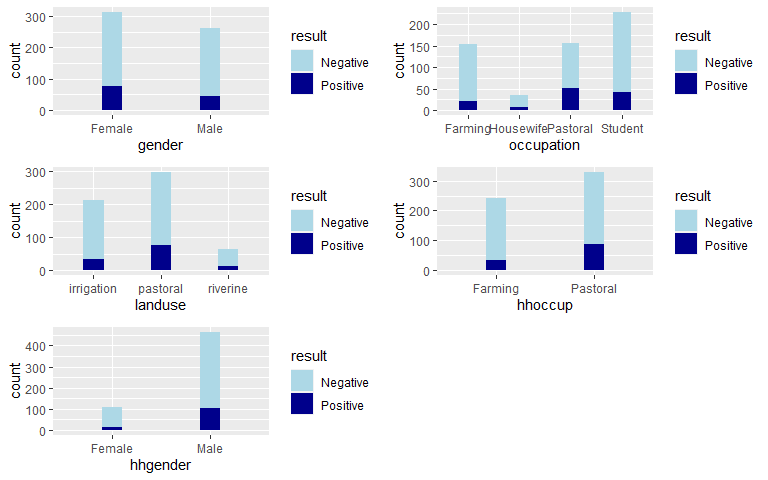
\includegraphics[width = \textwidth]{Images/factors.png}
	\caption{Stacked bar plot of \texttt{result} in factor variables}
	\label{fig:factor}
\end{figure}

\begin{table}
	\centering
	\begin{tabular}{|c|c|c|}
		\hline
		factor & category & prevalence \\
		\hline
		\multirow{2}{*}{\texttt{gender}} & Female & 0.2508 \\
		 & Male & 0.1821 \\
		\hline
		\multirow{4}{*}{\texttt{occupation}} & Farmer & 0.1465 \\
		 & Student & 0.1834 \\			
		 & Pastoralist & 0.3257 \\			
		 & Housewife & 0.2353 \\
		\hline
		\multirow{3}{*}{\texttt{landuse}} & irrigation & 0.1636 \\
		 & pastoral & 0.2597 \\
		 & riverine & 0.2090 \\
		\hline
		\multirow{2}{*}{\texttt{hhoccup}} & Farmer & 0.1325 \\
		 & Pastoralist & 0.2803 \\
		\hline
		\multirow{2}{*}{\texttt{hhgender}} & Female & 0.1481 \\
		 & Male & 0.2341 \\
		\hline
	\end{tabular}
	\caption{Prevalence in each category of factor variables}
	\label{tab:factor}
\end{table}

According to Figure \ref{fig:factor} and Table \ref{tab:factor}, \texttt{gender},  \texttt{occupation}, \texttt{landuse} and \texttt{hhoccup} have significantly different prevalence among categories, hence we select them as feature candidates in modelling step. Although it is also shown that prevalence between \texttt{hhgender} groups are significantly different, we do not include this column in our models as it is imbalanced distributed where over 80\% observations in this column are "Male".

\subsubsection{Numerical Variables}

We make box plots for numerical variables including \texttt{age}, \texttt{altitude}, \texttt{nmales}, \texttt{nfemales}, \texttt{famsize} and \texttt{disthosp}, grouped by \texttt{result}. Here, \texttt{altitude} denotes the altitude (recorded via GPS) of the village where the sample was collected, \texttt{nmales} and \texttt{nfemales} represent the number of males and females in the household sampled respectively, and \texttt{famsize}, the sum of \texttt{nmales} and \texttt{nfemales}, is the number of people in the sampled household. Note that there exists an observation with \texttt{disthosp} over 500 kilometres, which is deleted as an outlier, because the values of this feature in other observations from the same village are much lower.

\begin{figure}[!h]
	\centering
	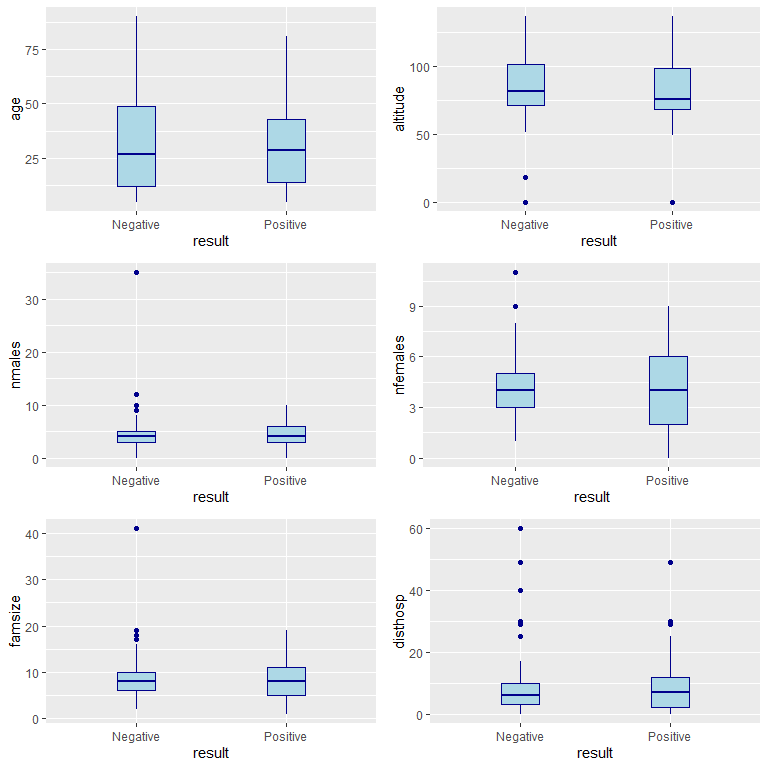
\includegraphics[width = 0.8\textwidth]{Images/numerical.png}
	\caption{Box plots of numerical variables, grouped by \texttt{result}}
	\label{fig:numerical}
\end{figure}

Comparing with factors, the distributions of numerical variables do not show significant difference between "Negative" and "Positive" groups from Figure \ref{fig:numerical}, which are probably insignificant in the models. Based on \cite{goarant2016leptospirosis}, we select \texttt{age}, \texttt{altitude}, \texttt{famsize} and \texttt{disthosp} as feature candidates for modelling. 

\subsubsection{Environmental Variables}

\texttt{village}, \texttt{location} and \texttt{constituency} are nominal variables indicating the geographical information of sampled people, with a nested order $\texttt{village} < \texttt{location} < \texttt{constituency}$.  As what we do for other nominal variables, we plot the stacked bar charts of the response variable and compute the prevalence, grouped by the levels in \texttt{village}, \texttt{location} and \texttt{constituency} respectively. 

\begin{figure}[!h]
	\centering
	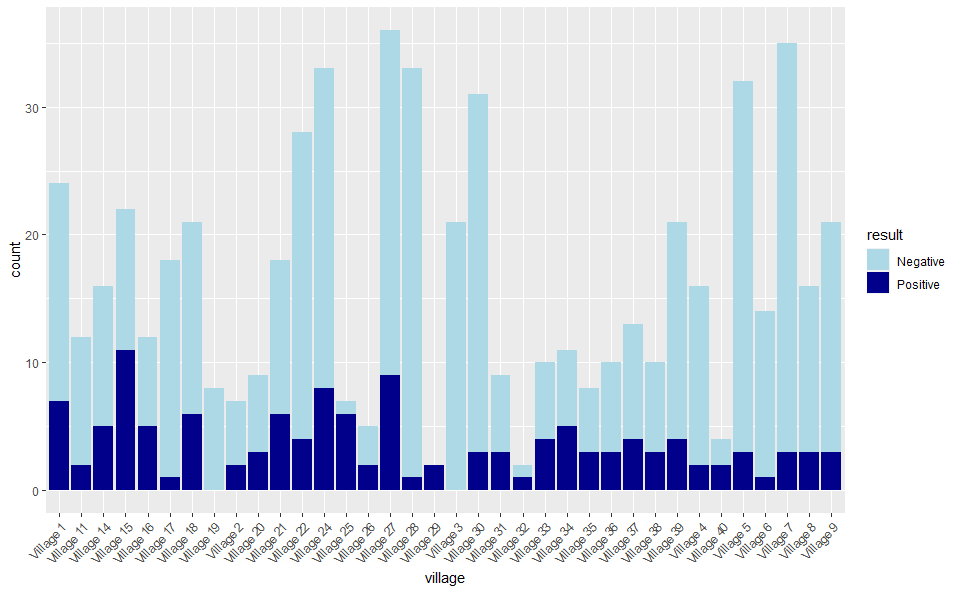
\includegraphics[width = 0.75\textwidth]{Images/village.png}
	\caption{Stacked bar plots of \texttt{result} in \texttt{village}}
	\label{fig:village} 
\end{figure}

\begin{table}[!h]
	\centering
	\begin{tabular}{|c|c|c|c|c|c|}
		\hline
		category & prevalence & category & prevalence & category & prevalence \\
		\hline
		Village 1 & 0.2917 & Village 16 & 0.4167 & Village 29 & 1.0000 \\
		Village 2 & 0.2857 & Village 17 & 0.0556 & Village 30 & 0.0968 \\
		Village 3 & 0 & Village 18 & 0.2857 & Village 31 & 0.3333 \\
		Village 4 & 0.1250 & Village 19 & 0 & Village 32 & 0.5000 \\
		Village 5 & 0.0938 & Village 20 & 0.3333 & Village 33 & 0.4000 \\
		Village 6 & 0.0714 & Village 21 & 0.3333 & Village 34 & 0.4545 \\
		Village 7 & 0.0857 & Village 22 & 0.1429 & Village 35 & 0.3750 \\
		Village 8 & 0.1875 & Village 24 & 0.2424 & Village 36 & 0.3000 \\		
		Village 9 & 0.1429 & Village 25 & 0.8571 & Village 37 & 0.3077 \\
		Village 11 & 0.1667 & Village 26 & 0.4000 & Village 38 & 0.3000 \\
		Village 14 & 0.3125 & Village 27 & 0.2500 &	Village 39 & 0.1905 \\
		Village 15 & 0.5000 & Village 2 & 0.0303 & Village 40 & 0.5000	\\
		\hline			
	\end{tabular}
	\caption{Prevalence in each category of \texttt{village}}
	\label{tab:village}
\end{table}

\begin{figure}[!h]
	\centering
	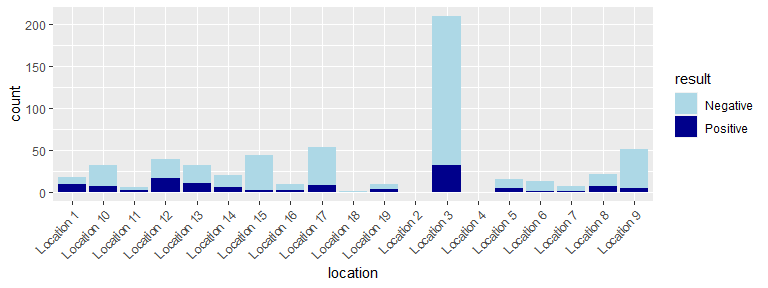
\includegraphics[width = 0.75\textwidth]{Images/location.png}
	\caption{Stacked bar plots of \texttt{result} in \texttt{location}}
	\label{fig:location}
\end{figure}

\begin{table}[!h]
	\centering
	\begin{tabular}{|c|c|c|c|c|c|}
		\hline
		category & prevalence & category & prevalence & category & prevalence \\
		\hline
		Location 1 & 0.5556 & Location 7 & 0.2857  & Location 13 & 0.3333 \\
		Location 2 & 1.0000	 & Location 8 & 0.3182 & Location 14 & 0.2857 \\
		Location 3 & 0.1571 & Location 9 & 0.0962 & Location 15 & 0.0667 \\
		Location 4 & 1.0000 & Location 10 & 0.2424 & Location 16 & 0.3000 \\
		Location 5 & 0.3125 & Location 11 & 0.5000 & Location 17 & 0.1667 \\
		Location 6 & 0.1429 & Location 12 & 0.4250 & Location 18 & 0.0000 \\
		 & & & & Location 19 & 0.4000 \\	
		\hline			
	\end{tabular}
	\caption{Prevalence in each category of \texttt{location}}
	\label{tab:location}
\end{table}

\begin{figure}[!h]
	\centering
	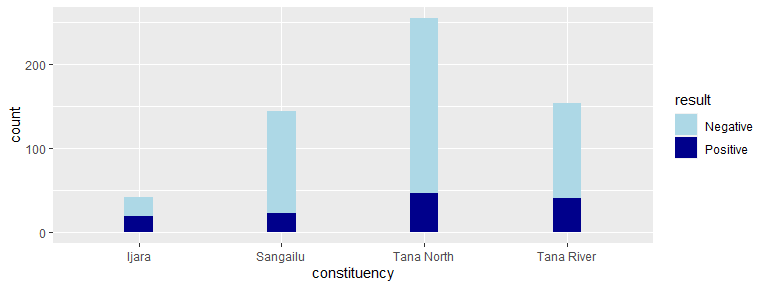
\includegraphics[width = 0.75\textwidth]{Images/constituency.png}
	\caption{Stacked bar plots of \texttt{result} in \texttt{constituency}}
	\label{fig:constituency}
\end{figure}	

\begin{table}[!h]
	\centering
	\begin{tabular}{|c|c|c|c|}
		\hline
		category & prevalence & category & prevalence \\
		\hline
		Tana North & 0.1843 & Tana River & 0.2662 \\
		Ijara & 0.4524 & Sangailu & 0.1597 \\
		\hline			
	\end{tabular}
	\caption{Prevalence in each category of \texttt{constituency}}
	\label{tab:constituency}
\end{table}

According to the plots and tables, we may also consider the influence of these geographical variables on Leptospirosis diagnosis in our models due to different prevalence among groups. However, \texttt{village} and \texttt{location} contain a number of levels, which causes great model complexity with high degrees of freedom and further unstable estimates. Thus, we consider the models with the random effect of these geographical variables. The details of random effect will be explained in the next section.

Up to now, we have extracted a subset for modelling with 595 observations left and 11 feature candidates, including 4 nominal variables, 4 numerical variables and 3 geographical variables.

\clearpage

\section{Implementation}
\label{sec:implementation}

In this section, we introduce the definition and purpose of General Linear Mixed Model (GLMM) with random effect used for modelling. Moreover, we explain the model construction , and further the comparison among models.

\subsection{General Linear Mixed Model}

The exposition in this subsection follows that in Zuur (2009) \cite{zuur2009}.

\subsection{Model Construction and Selection}

\subsubsection{Step 1: Initial Model}

Following Zuur's logic, we start with a binomial GLM, i.e. logistic regression, containing all feature candidates excluding geographical variables. Here, we do not contain the interaction terms of variables in the model as we do not detect much interaction existing among features in EDA section. On the other hand, introducing interaction terms increases much model complexity due to a large number of potential interaction terms. 

\subsubsection{Step 2: Find the Optimal Fixed Structure}

The \texttt{summary} function and \texttt{step} function are both used to determine variables with the optimal fixed effect among candidates. The former function obtains the feature significance based on the $t$ test, while the latter one choose the optimal model and significant features by AIC and the $\chi^2$ test. Table \ref{tab:summary1} show the significance of features in the initial GLM based on \texttt{summary} function, and Table \ref{tab:step1} display the significant features based on \texttt{step} function.

\begin{table}[!h]
	\centering
	\begin{tabular}{|c|c|c|}
		\hline
		 & $t$ value & Pr($>|z|$) \\
		\hline
		\texttt{(Intercept)} & -0.341 & 0.73317 \\
		\texttt{genderMale} & -2.428 & \ \ \ 0.01520 * \\
		\texttt{age} & -1.798 & \ \ 0.07219 . \\
		\texttt{occupationHousewife} & -0.757 & 0.44890 \\  
		\texttt{occupationPastoralist} & 0.754 & 0.45068 \\   
		\texttt{occupationStudent} & -1.423 & 0.15463 \\  
		\texttt{landusepastoral} & -2.347 & \ \ \ 0.01892 * \\ 
		\texttt{landuseriverine} & -1.607 & 0.10810 \\   
		\texttt{altitude} & -1.681 & \ \ 0.09283 . \\
		\texttt{famsize} & 0.346 & 0.72900 \\   
		\texttt{hhoccupPastoralist} & 3.181 & \ \ \ \ 0.00147 ** \\
		\texttt{disthosp} & 0.301 & 0.76322 \\   
		\hline
		\multicolumn{3}{|l|}{Significance codes: 0,\ ‘***’ 0.001,\ ‘**’ 0.01,\ ‘*’ 0.05,\ ‘.’ 0.1,\ ‘ ’ 1} \\
		\hline
	\end{tabular}
	\caption{Feature significance in initial GLM using \texttt{summary} function}
	\label{tab:summary1}
\end{table}

\begin{table}[!h]
	\centering
	\begin{tabular}{|c|c|c|c|}
		\hline
		 & Df & AIC & Pr($>$Chi) \\
		\hline
		\texttt{(none)} & & 602.72 & \\                      
		\texttt{altitude} & 1 & 603.45 & 0.0990659 . \\ 
		\texttt{age} & 1 & 603.86 & 0.0765869 . \\ 
		\texttt{landuse} & 2 & 604.59 & 0.0531339 . \\ 
		\texttt{occupation} & 3 & 605.55 & \ 0.0316715 * \\ 
		\texttt{gender} & 1 & 606.75 & \ 0.0141019 * \\ 
		\texttt{hhoccup} & 1 & 611.90 & \ \ \ \ 0.0008302 *** \\
		\hline
		\multicolumn{4}{|l|}{Significance codes: 0,\ ‘***’ 0.001,\ ‘**’ 0.01,\ ‘*’ 0.05,\ ‘.’ 0.1,\ ‘ ’ 1} \\
		\hline
	\end{tabular}
	\caption{Significant features in stepwise algorithm using \texttt{step} function}
	\label{tab:step1}
\end{table}

Based on two tables, we select \texttt{gender} and \texttt{hhoccup} in further steps, which are both statistically significant at 0.05 significance level in two function results. Besides, \texttt{landuse} is also selected in fixed structure,  as it is significant at 0.1 significance level in stepwise selection and its level is statistically significant at 0.05 level in model summary.  

Although \texttt{occupation} shows its significance in stepwise algorithm, none of its levels is significant in model summary. Moreover, as mentioned in EDA section, we observe high correlation between \texttt{occupation} and \texttt{landuse}, which probably causes the problem of collinearity and poor model performance. Therefore, we do not include \texttt{occupation} in the fixed structure.

In conclusion, the optimal fixed structure consists of \texttt{gender}, \texttt{landuse} and \texttt{hhoccup}.

\subsubsection{Step 3: Find the Optimal Random Structure}

With the pre-determined fixed structure, we now introduce the random effect of geographical variables and determine GLMM with the best performance, using R package \texttt{lme4} \cite{lme4}. As mentioned, we consider the random effect of \texttt{village} and \texttt{location} to investigate whether there is a village or location effect. 

We start with fitting the random intercept model of \texttt{village}. To assess whether the model with mixed effect model is better than the ordinary binomial GLM, we refit the latter one over the selected features without random intercept and compare the models using \texttt{anova} function. The output is given in Table \ref{tab:glmm1}:

\begin{table}[!h]
	\centering
	\begin{tabular}{|c|c|c|c|c|c|c|c|c|}
		\hline
		 & npar & AIC & BIC & logLik & deviance & Chisq & Df & Pr($>$Chisq) \\  
		 \hline
		GLM & 5 & 603.63 & 625.57 & -296.81 & 593.63 & & & \\                      
		GLMM(\texttt{village}) & 6 & 601.87 & 628.20 & -294.93 & 589.87 & 3.7611 & 1 & 0.05246 . \\
		\hline
		\multicolumn{9}{|l|}{Significance codes: 0,\ ‘***’ 0.001,\ ‘**’ 0.01,\ ‘*’ 0.05,\ ‘.’ 0.1,\ ‘ ’ 1} \\
		\hline
	\end{tabular}
	\caption{Comparison between GLM and GLMM of \texttt{village}}
	\label{tab:glmm1}
\end{table}

The lower AIC value in the table indicate that the mixed model including the random effect of village is preferred. Moreover, we extend the random part by building random intercept and slope models. Specifically, the \texttt{landuse} effect may be different per village, and the same may hold for the \texttt{hhoccup} effect. Table \ref{tab:glmm2} show the output of model comparison using \texttt{anova} function:

\begin{table}[!h]
	\centering
	\begin{tabular}{|c|c|c|c|c|c|c|c|c|}
		\hline
		& npar & AIC & BIC & logLik & deviance & Chisq & Df & Pr($>$Chisq) \\  
		\hline
		random intercept & 6 & 601.87 & 628.20 & -294.93 & 589.87 & & & \\                      
		random intercept + \texttt{landuse} & 8 & 605.75 & 640.85 & -294.87 & 589.75 & 0.122 & 2 & 0.9408 \\
		random intercept + \texttt{hhoccup} & 11 & 611.48 & 659.76 & -294.74 & 589.48 & 0.264 & 3 & 0.9667 \\
		\hline
		\multicolumn{9}{|l|}{Significance codes: 0,\ ‘***’ 0.001,\ ‘**’ 0.01,\ ‘*’ 0.05,\ ‘.’ 0.1,\ ‘ ’ 1} \\
		\hline
	\end{tabular}
	\caption{Comparison among GLMMs of \texttt{village} with different random structures}
	\label{tab:glmm2}
\end{table}

Extending the model with random slopes gives no improvement as the AIC values of models with random slopes get higher. Now we look at the alternative random intercept model considering the location effect. Comparison between random intercept models of \texttt{village} and \texttt{location} using \texttt{AIC} command is displayed in Table \ref{tab:glmm3}:

\begin{table}[!h]
	\centering
	\begin{tabular}{|c|c|c|}
		\hline
		& df & AIC  \\  
		\hline
		GLMM(\texttt{village}) & 6 & 576.9177	\\	
		GLMM(\texttt{location}) & 6 & 577.3410 \\
		\hline
	\end{tabular}
	\caption{Comparison between random intercept models of \texttt{village} and \texttt{location}}
	\label{tab:glmm3}
\end{table}

According to the table, the AIC value of the random intercept model with the village effect is slightly lower. Besides, since the column \texttt{village} contains more levels than \texttt{location}, the models considering the random effect on village aspect obtain more detailed results. Moreover, the random intercept and slope models of \texttt{location} perform even worse. As a result, we prefer the random intercept model with village effect.

\

Note that here we do not consider the constituency effect in our model as \texttt{constituency} only contains 4 levels. It may be better to include this variable in model's fixed structure. However, after introducing the fixed effect of \texttt{constituency}, other variables in the fixed structure become insignificant. Moreover, the variance and standard deviation of the random effect of \texttt{village} or \texttt{location} turn to 0, indicating the insignificance of random effect. Further details are given in Appendix. Consequently, the influence of \texttt{constituency} is ruled out.

\clearpage

\section{Results}
\label{sec:results}

The random intercept model with \textbf{village} effect is determined as the optimal model, given by:
\begin{align*}
	Y_{ij} & \sim Binomial(1, p_{ij}) \\
	logit(p_{ij}) &=  -1.5997 - 0.4711 \times \mathbb{I}(\texttt{gender}_{ij} = Male)  \\
					      & \ \ \ \ - 0.9956 \times \mathbb{I}(\texttt{landuse}_{ij} = pastoral) - 0.4744 \times \mathbb{I}(\texttt{landuse}_{ij} = riverine) \\
					      & \ \ \ \ + 1.7649 \times \mathbb{I}(\texttt{hhoccup}_{ij} = Pastoralist) + v_{ij} \\
	v_i & \sim Normal(0, 0.2553^2)
\end{align*}	

Here, the index $i$ refers to villages and $j$ to the observation within a village. Moreover, $v_i$ denotes the random intercept across villages.

Before any interpretation, we carry out the diagnosis and evaluation of the optimal model.

\subsection{Model Diagnosis} 

According to \cite{zuur2009mixed}, model diagnosis is required once we obtain the optimal model. In linear regressions, we usually look at the corresponding residual plots and normal Q-Q plots to check if the linearity assumption and the normality of error terms are satisfied. However, these are probably not suitable for GL(M)Ms. Standard residual plots, when interpreted in the same way as for linear models, seem to show all kind of problems, such as non-normality, heteroscedasticity, even if the model is correctly specified. For example, the standard residual plot of our optimal model, shown in Figure \ref{fig:std_resplot}, has an obvious pattern. In this case, we get confused and are not able to tell whether such pattern in GLMM residuals is a problem or not.

\begin{figure}[!h]
	\centering
	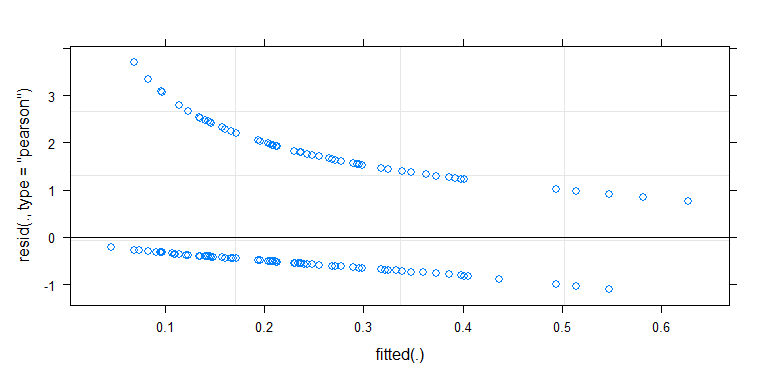
\includegraphics[width = 0.75\textwidth]{Images/std_resplot.png}
	\caption{Standard residual plot of the optimal model}
	\label{fig:std_resplot}
\end{figure}

To address this problem, we adopt the \texttt{DHARMa} package \cite{dharma}. This package aims to create readily interpretable residuals for GL(M)Ms that are standardized to values between 0 and 1. \texttt{DHARMa} also provides Q-Q plots to detect overall deviations from the expected distribution, by default with added tests for correct distribution (Kolmogorov-Smirnov test), dispersion and outliers. The use of simulation-based approach ensures the strength of diagnosis results. The basic steps \cite{dharma} are:

\begin{enumerate}
	\item Simulate new response data from the fitted model for each observation.
	\item For each observation, calculate the empirical cumulative density function for the simulated observations, which describes the possible values (and their probability) at the predictor combination of the observed value, assuming the fitted model is correct.
	\item The residual is defined as the value of the empirical density function at the value of the observed data.
\end{enumerate}

Therefore, we simulate 1000 observations based on our optimal model, and plot the scaled residuals.

\begin{figure}[!h]
	\centering
	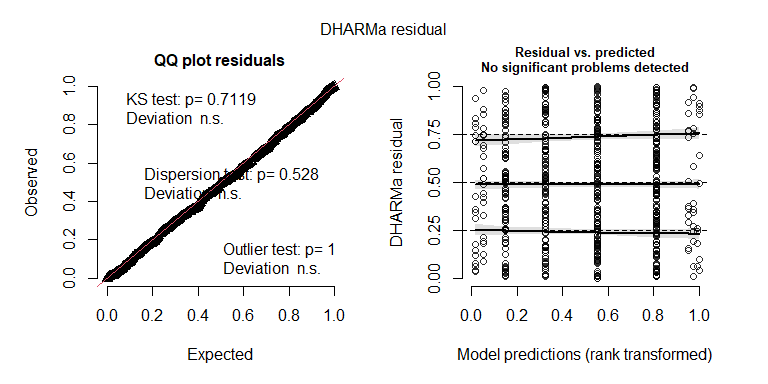
\includegraphics[width = 0.75\textwidth]{Images/diagnosis1.png}
	\caption{\texttt{DHARMa} residual plot and Q-Q plot of the optimal model}
	\label{fig:diagnosis1}
\end{figure}

Intuitively, nothing in the Figure \ref{fig:diagnosis1} is highlighted in red, indicating no violation of model assumptions is detected. Specifically, we observe the scaled residuals fall along the straight line at 45-degree angle in the Q-Q plot, hence we obtain that the residuals are normally distributed. Moreover, we cannot reject the null hypothesis of KS test that the observed distribution of scaled residuals is the same as the expected distribution, due to the p-value of 0.7119. Large p-values in dispersion test and outlier test also indicate no problem of overdispersion or outlier. In the residual plot on the right, we do not observe obvious pattern of residuals. The empirical 0.25, 0.5 and 0.75 quantiles does not show significant deviation from the theoretical quartiles, suggesting the uniformity in y-direction holds. As a result, we do not detect significant problems in the optimal model.

It is highly recommended in \cite{dharma} to plot residuals against a specific predictor. Here, we plot the scaled residuals of \texttt{landuse}, one of the fixed effects in the optimal model, and \texttt{occupation}, one of the verbalises excluded from the model. Again, we do not find significant problems in Figure \ref{fig:diagnosis2}. Thus, the assumptions of the optimal model are satisfied.

\begin{figure}[!h]
	\centering
	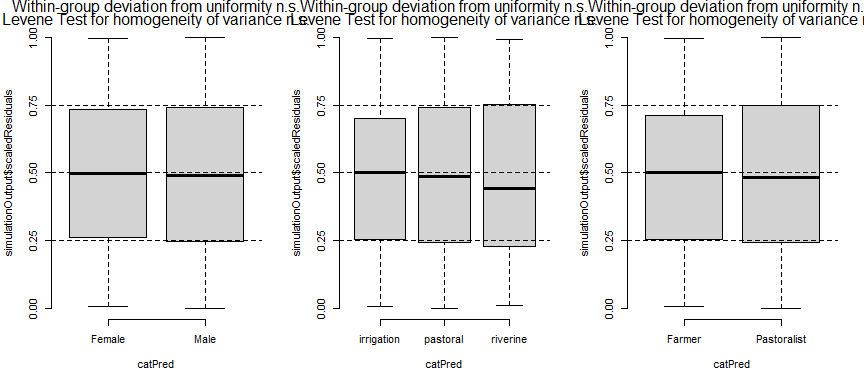
\includegraphics[width = 0.75\textwidth]{Images/diagnosis2.png}
	\caption{\texttt{DHARMa} residual plots of \texttt{landuse} (left) and \texttt{occupation} (right)}
	\label{fig:diagnosis2}	
\end{figure} 

\subsection{Model Evaluation}

Since the response of our model is binomial, for model evaluation, we plot the ROC (Receiver Operating Characteristic) curve of the optimal model and compute the corresponding AUC (Area Under Curve) value with 95\% confidence intervals. We repeat the same steps for the ordinary GLM and the random intercept model with location effect. 

\begin{figure}[!h]
	\centering
	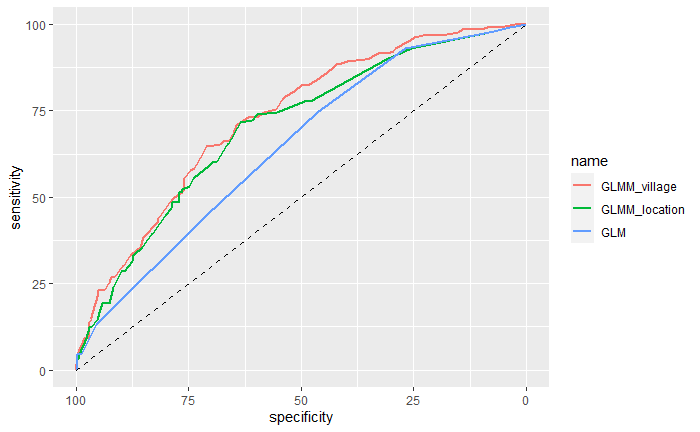
\includegraphics[width = 0.75\textwidth]{Images/ROC.png}
	\caption{ROC curves of models} 
	\label{fig:pROC}
\end{figure}

\begin{table}[!h]
	\centering
	\begin{tabular}{|c|c|c|}
		\hline
		 & AUC & 95\% CI \\
		\hline
		GLMM(\texttt{village}) & 0.7275 & (0.6806, 0.7745) \\
		GLMM(\texttt{location}) & 0.7018 & (0.6520, 0.7516) \\
		GLM & 0.6437 & (0.5942, 0.6932) \\
		\hline	
	\end{tabular}
	\caption{AUC values with 95\% confidence intervals of models}
	\label{tab:AUC}
\end{table}

According to Figure \ref{fig:pROC} and Table \ref{tab:AUC}, ROC curve beyond the random guess line and AUC value of 0.7275, which is larger than 0.5, indicate better performance of the optimal model than the random classifier. Moreover, the random intercept model with village effect over-performs the rest two models, implying its better ability to explain and predict. 

Furthermore, we compute the mean AUC of models using 10-fold cross validation. As shown in Table \ref{tab:meanAUC}, again, the optimal model performs the best among three models.

\begin{table}[!h]
	\centering
	\begin{tabular}{|c|c|}
		\hline
		 & mean AUC \\
		\hline
		GLMM (\texttt{village}) & 0.6687 \\
		GLMM (\texttt{location}) & 0.6681 \\
		GLM & 0.6454 \\
		\hline
	\end{tabular}
	\caption{Mean AUC of models based on 10-fold cross validation}
	\label{tab:meanAUC}
\end{table}

\subsection{Model Interpretation}

\clearpage

\section{Conclusions}

We construct a modified Bayesian network on a subset of easySHARE dataset to identify risk factors on dementia. As a result, age, gender, country, education and depression tend to have significant influence on individual's cognitive function. Specifically, the probability of severe cognitive impairment rises as age or depression level increases. In particular, individuals over 65 years old or experiencing high-level depression have much higher dementia risk. Education shows opposite influence on cognitive function that people with higher education levels have lower risk. Gender and country affect individual's cognition in a variety of ways. Generally, females have higher dementia risk than males; people from countries with low aGDP have higher probability to suffer from dementia.

There are some limitations of this research. First, although hearing loss, diabetes, and hypertension are believed to have important effect on cognitive impairment in \cite{livingston2017dementia}, their influence could not be identified due to the lack of relevant columns in easySHARE data. We could only define a general factor "chronic diseases" to count the number of chronic diseases the respondents had and explore its possible influence on dementia risk instead. To determine the specific effects of these diseases, we need to access data with relevant variables. Second, our research belongs to cross-sectional analysis, which focuses on data at a specific time point among different individuals and obtains conclusions for the general population. In this case, our research is lack of the exploration on longitudinal effects of some risk factors on dementia risk among particular respondents over the time.

\clearpage

%the entries have to be in the file literature.bib
\bibliographystyle{unsrt}
\bibliography{literature}
\clearpage

\appendix
\section*{Appendix}
\addcontentsline{toc}{section}{Appendix}

Programming part in this research is completed with R. 

\subsection*{R packages:}

For EDA section, we use the \texttt{tidyverse} and \texttt{gridExtra} packages. We construct and estimate the networks with \texttt{bnlearn} package and display the network with \texttt{Rgraphviz} package. \texttt{MASS} package is used to fit the ordered logistic regression on cognitive score. All histograms and line graphs are generated with \texttt{ggplot2}.

\subsection*{R code: }
The complete code is available via this \href{https://github.com/Shi-Yile/Project-1-Dementia-Risk-Factors.git}{Github repository}.

\clearpage

\section*{Word Count}
\addcontentsline{toc}{section}{Word Count}

This report contains 4828 words, including executive summary, main text, references and appendix. The screenshot using  \texttt{Analyse Text} function in TeXstudio is provided.

\end{document}
